\subsection{The U-boot bootloader}

\begin{frame}
  \frametitle{U-Boot}
  \begin{columns}
    \column{0.7\textwidth}
      U-Boot is a typical free software project
      \begin{itemize}
      \item License: GPLv2 (same as Linux)
      \item Freely available at \url{https://www.denx.de/wiki/U-Boot}
      \item Documentation available at
        \url{https://u-boot.readthedocs.io/en/latest/}
      \item The latest development source code is available in a Git
        repository:
        \url{https://gitlab.denx.de/u-boot/u-boot}
      \item Development and discussions happen around an open mailing-list
        \url{https://lists.denx.de/pipermail/u-boot/}
      \item Follows a regular release schedule. Every 2 or 3 months,
        a new version is released. Versions are named \code{YYYY.MM}.
      \end{itemize}
    \column{0.3\textwidth}
      \includegraphics[width=\textwidth]{slides/sysdev-bootloaders-u-boot/u-boot-logo.pdf}\\
      \tiny Image credits: \url{https://frama.link/rwCUFc-T}
  \end{columns}
\end{frame}

\begin{frame}
  \frametitle{U-Boot configuration}
  \begin{itemize}
  \item Get the source code from the website or from git
  \item The \projdir{u-boot}{configs} directory contains one or several
        configuration file(s) for each supported board
    \begin{itemize}
    \item It defines the CPU type, the peripherals and their configuration, the
      memory mapping, the U-Boot features that should be compiled in, etc.
     \item Examples:\\
           \projfile{u-boot}{configs/stm32mp15_basic_defconfig}\\
           \projfile{u-boot}{configs/stm32mp15_trusted_defconfig}
    \end{itemize}
  \item Note: U-Boot is migrating from board configuration defined in
    C header files (\projdir{u-boot}{include/configs}) to {\em defconfig} like in
    the Linux kernel (\projdir{u-boot}{configs})
    \begin{itemize}
    \item Not all boards have been converted to the new configuration
      system.
    \item Many boards still have {\em both} hardcoded configuration settings in
          \code{.h} files, and configuration settings in \code{defconfig}
          files that can be overriden with configuration interfaces.
    \end{itemize}
  \end{itemize}
\end{frame}

\begin{frame}[fragile]
  \frametitle{U-Boot configuration file}
\begin{block}{CHIP\_defconfig}
\begin{Verbatim}[formatcom=\tiny\ttfamily]
CONFIG_ARM=y
CONFIG_ARCH_SUNXI=y
CONFIG_MACH_SUN5I=y
CONFIG_DRAM_TIMINGS_DDR3_800E_1066G_1333J=y
# CONFIG_MMC is not set
CONFIG_USB0_VBUS_PIN="PB10"
CONFIG_VIDEO_COMPOSITE=y
CONFIG_DEFAULT_DEVICE_TREE="sun5i-r8-chip"
CONFIG_SPL=y
CONFIG_SYS_EXTRA_OPTIONS="CONS_INDEX=2"
# CONFIG_CMD_IMLS is not set
CONFIG_CMD_DFU=y
CONFIG_CMD_USB_MASS_STORAGE=y
CONFIG_AXP_ALDO3_VOLT=3300
CONFIG_AXP_ALDO4_VOLT=3300
CONFIG_USB_MUSB_GADGET=y
CONFIG_USB_GADGET=y
CONFIG_USB_GADGET_DOWNLOAD=y
CONFIG_G_DNL_MANUFACTURER="Allwinner Technology"
CONFIG_G_DNL_VENDOR_NUM=0x1f3a
CONFIG_G_DNL_PRODUCT_NUM=0x1010
CONFIG_USB_EHCI_HCD=y
\end{Verbatim}
\end{block}
\end{frame}

\begin{frame}
  \frametitle{Configuring and compiling U-Boot}
  \begin{itemize}
  \item U-Boot must be configured before being compiled
    \begin{itemize}
    \item Configuration stored in a \code{.config} file
    \item \code{make BOARDNAME_defconfig}
    \item Where \code{BOARDNAME} is the name of a configuration, as
      visible in the \code{configs/} directory.
    \item You can then run \code{make menuconfig} to further customize
      U-Boot's configuration!
    \end{itemize}
  \item Make sure that the cross-compiler is available in \code{PATH}
  \item Compile U-Boot, by specifying the cross-compiler prefix.\\
    Example, if your cross-compiler executable is \code{arm-linux-gcc}:\\
    \code{make CROSS_COMPILE=arm-linux-}
  \item The main result is a \code{u-boot.bin} file, which is the
    U-Boot image. Depending on your specific platform, or what storage
    device you're booting from (NAND or MMC), there may be
    other specialized images: \code{u-boot.img}, \code{u-boot.kwb}...
  \item This also generates the U-Boot SPL image to be flashed
    together with U-Boot. The exact file name can vary too, depending
    on what the romcode expects.
  \end{itemize}
\end{frame}

\begin{frame}
  \frametitle{Installing U-Boot}
  U-Boot must usually be installed in flash memory to be
  executed by the hardware. Depending on the hardware, the
  installation of U-Boot is done in a different way:
  \begin{itemize}
  \item The CPU provides some kind of specific boot monitor with
    which you can communicate through the serial port or USB using a
    specific protocol
  \item The CPU boots first on removable media (MMC) before booting
    from fixed media (NAND). In this case, boot from MMC to reflash
    a new version
  \item U-Boot is already installed, and can be used to flash a new
    version of U-Boot. However, be careful: if the new version of
    U-Boot doesn't work, the board is unusable
  \item The board provides a JTAG interface, which allows to write
    to the flash memory remotely, without any system running on the
    board. It also allows to rescue a board if the bootloader
    doesn't work.
  \end{itemize}
\end{frame}

\begin{frame}[fragile]
  \frametitle{U-boot prompt}
  \begin{itemize}
  \item Connect the target to the host through a serial console.
  \item Power-up the board. On the serial console, you will see
        something like:
  \end{itemize}
\tiny
\begin{verbatim}
U-Boot 2020.04 (May 26 2020 - 16:05:43 +0200)

CPU: SAMA5D36
Crystal frequency:       12 MHz
CPU clock        :      528 MHz
Master clock     :      132 MHz
DRAM:  256 MiB
NAND:  256 MiB
MMC:   Atmel mci: 0, Atmel mci: 1
Loading Environment from NAND... OK
In:    serial@ffffee00
Out:   serial@ffffee00
Err:   serial@ffffee00
Net:   eth0: ethernet@f0028000
Error: ethernet@f802c000 address not set.

Hit any key to stop autoboot:  0
=>
\end{verbatim}
\normalsize
  \begin{itemize}
  \item The U-Boot shell offers a set of commands. We will study the
    most important ones, see the documentation for a complete
    reference or the \code{help} command.
  \end{itemize}
\end{frame}

\begin{frame}[fragile]
  \frametitle{Information commands}
\begin{block}{Version details}
{\tiny
\begin{verbatim}
=> version
U-Boot 2020.04 (May 26 2020 - 16:05:43 +0200)

arm-linux-gcc (crosstool-NG 1.24.0.105_5659366) 9.2.0
GNU ld (crosstool-NG 1.24.0.105_5659366) 2.34
\end{verbatim}}
\end{block}

\begin{block}{NAND flash information}
{\tiny
\begin{verbatim}
=> nand info

Device 0: nand0, sector size 128 KiB
  Page size       2048 b
  OOB size          64 b
  Erase size    131072 b
  subpagesize     2048 b
  options     0x40004200
  bbt options 0x00008000
\end{verbatim}}
\end{block}
\end{frame}

\begin{frame}
  \frametitle{Important commands (1)}
  \begin{itemize}
  \item The exact set of commands depends on the U-Boot configuration
  \item \code{help} and \code{help command}
  \item \code{fatload}, loads a file from a FAT filesystem to RAM
    \begin{itemize}
    \item Example: \code{fatload usb 0:1 0x21000000 zImage}
    \item And also \code{fatinfo}, \code{fatls}, \code{fatsize},
          \code{fatwrite}...
    \end{itemize}
  \item Similar commands for other filesystems: \code{ext2load}, \code{ext2ls},
      \code{ext4load}, \code{ext4ls}, \code{sqfsload}, \code{sqfsls}...
      (\href{https://bootlin.com/blog/bootlin-contributes-squashfs-support-to-u-boot/}{SquashFS
      support contributed by Bootlin})
  \item Note that filesystem independent commands such as \code{load},
        \code{ls}, and \code{size} exist. Examples:
    \begin{itemize}
    \item \code{load usb 0:1 0x21000000 zImage}
    \item \code{ls mmc 0:2 boot/}
    \item \code{size mmc 0:1 dtb} (result stored in \code{filesize} environment variable)
    \end{itemize}
  \item \code{loadb}, \code{loads}, \code{loady}, load a file from the
    serial line to RAM
  \item \code{tftp}, loads a file from the network to RAM (example given later)
  \end{itemize}
\end{frame}

\begin{frame}
  \frametitle{Important commands (2)}
  \begin{itemize}
  \item \code{ping}, to test the network
  \item \code{bootd} (can be abbreviated as \code{boot}), runs the default
    boot command, stored in the \code{bootcmd} environment variable (explained later)
  \item \code{bootz <address>}, starts a compressed kernel image loaded at the
    given address in RAM
  \item \code{usb}, to initialize and control the USB subsystem,
    mainly used for USB storage devices such as USB keys
  \item \code{mmc}, to initialize and control the MMC subsystem, used
    for SD and microSD cards
  \item \code{nand}, to erase, read and write contents to NAND flash
  \item \code{md}, displays memory contents. Can be useful to check the
    contents loaded in memory, or to look at hardware registers.
  \item \code{mm}, modifies memory contents. Can be useful to modify
    directly hardware registers, for testing purposes.
\end{itemize}
\end{frame}

\begin{frame}
  \frametitle{U-Boot bdinfo command}
  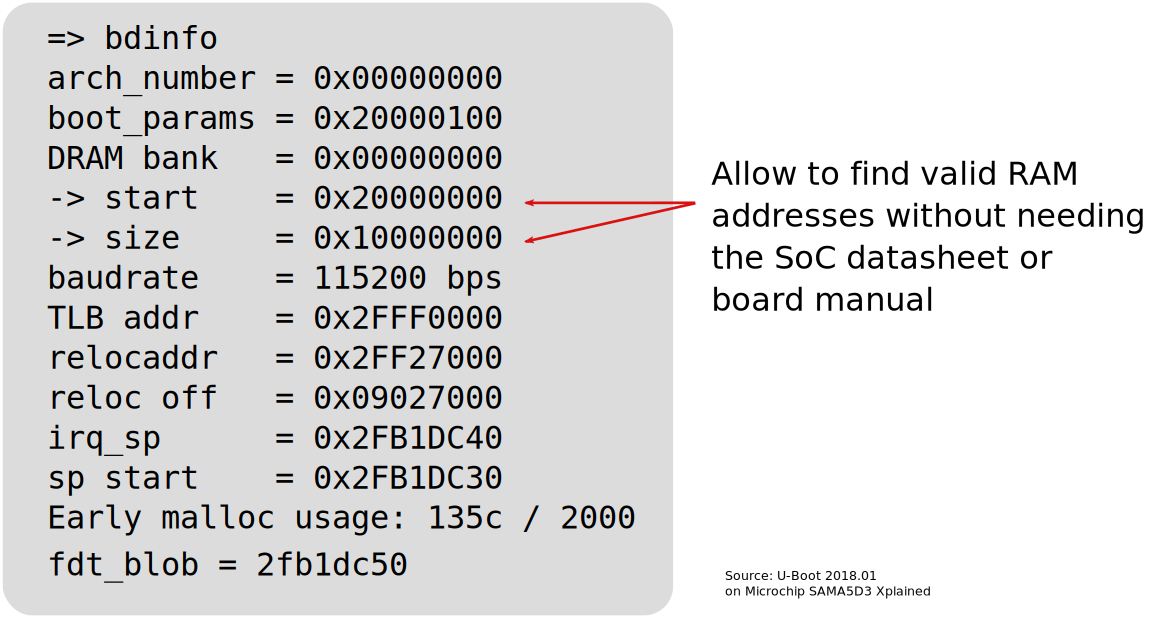
\includegraphics[height=0.85\textheight]{slides/sysdev-bootloaders-u-boot/u-boot-bdinfo.pdf}
\end{frame}

\begin{frame}
  \frametitle{Environment variables: principle}
  \begin{itemize}
  \item U-Boot can be configured through environment variables
    \begin{itemize}
    \item Some specific environment variables impact the behavior of
      the different commands
    \item Custom environment variables can be added, and used in
      scripts
    \end{itemize}
  \item Environment variables are loaded from persistent storage to RAM at U-Boot
    startup. They can be defined or modified and saved back to storage
    for persistence.
  \end{itemize}
\end{frame}

\begin{frame}
  \frametitle{Environment variables: implementation}
  \begin{columns}
  \column{0.5\textwidth}
    Depending on the configuration, the U-Boot environment is typically stored in:
    \begin{itemize}
	  \item At a fixed offset in NAND flash
	  \item At a fixed offset on MMC or USB storage, before the beginning of
                the first partition.
	  \item In a file (\code{uboot.env}) on a FAT or ext4 partition
	  \item In a UBI volume
    \end{itemize}
  \column{0.5\textwidth}
    \includegraphics[width=\textwidth]{slides/sysdev-bootloaders-u-boot/u-boot-environment-configuration.png}\\
    \vspace{0.3cm}
    \tiny U-Boot environment configuration menu
  \end{columns}
\end{frame}

\begin{frame}
  \frametitle{Environment variables commands}
  Commands to manipulate environment variables:
  \begin{itemize}
    \item \code{printenv}\\
      Shows all variables
    \item \code{printenv <variable-name>}\\
      Shows the value of a variable
    \item \code{setenv <variable-name> <variable-value>}\\
      Changes the value of a variable or defines a new one, only in RAM
    \item \code{editenv <variable-name>}\\
      Edits the value of a variable in-place, only in RAM
    \item \code{saveenv}\\
      Saves the current state of the environment to storage for persistence.
  \end{itemize}
\end{frame}

\begin{frame}[fragile]
\frametitle{Environment variables commands - Example}
\small
\begin{verbatim}
=> printenv
baudrate=19200
ethaddr=00:40:95:36:35:33
netmask=255.255.255.0
ipaddr=10.0.0.11
serverip=10.0.0.1
stdin=serial
stdout=serial
stderr=serial
=> setenv serverip 10.0.0.100
=> printenv serverip
serverip=10.0.0.100
=> saveenv
\end{verbatim}
\end{frame}

\begin{frame}
  \frametitle{Important U-Boot env variables}
  \begin{itemize}
  \item \code{bootcmd}, specifies the commands that U-Boot will
    automatically execute at boot time after a configurable delay
    (\code{bootdelay}), if the process is not interrupted. See next
    page for an example.
  \item \code{bootargs}, contains the arguments passed to the Linux
    kernel, covered later
  \item \code{serverip}, the IP address of the server that U-Boot will
    contact for network related commands
  \item \code{ipaddr}, the IP address that U-Boot will use
  \item \code{netmask}, the network mask to contact the server
  \item \code{ethaddr}, the MAC address, can only be set once
  \item \code{filesize}, the size of the latest copy to memory
    (from \code{tftp}, \code{fatload}, \code{nand read}...)
  \end{itemize}
\end{frame}

\begin{frame}
  \frametitle{Scripts in environment variables}
  \begin{itemize}
  \item Environment variables can contain small scripts, to execute
    several commands and test the results of commands.
    \begin{itemize}
    \item Useful to automate booting or upgrade processes
    \item Several commands can be chained using the \code{;} operator
    \item Tests can be done using
      \code{if command ; then ... ; else ... ; fi}
    \item Scripts are executed using \code{run <variable-name>}
    \item You can reference other variables using
      \code{${variable-name}}
    \end{itemize}
  \item Examples
    \begin{itemize}
    \item \code{setenv bootcmd 'tftp 0x21000000 zImage; tftp 0x22000000 dtb; bootz 0x21000000 - 0x22000000'}
    \item \code{setenv mmc-boot 'if fatload mmc 0 80000000
      boot.ini; then source; else if fatload mmc 0 80000000 zImage;
      then run mmc-do-boot; fi; fi'}
  \end{itemize}
\end{itemize}
\end{frame}

\begin{frame}
  \frametitle{Transferring files to the target}
  \begin{itemize}
  \item U-Boot is mostly used to load and boot a kernel image, but it
    also allows to change the kernel image and the root filesystem
    stored in flash.
  \item Files must be exchanged between the target and the development
    workstation. This is possible:
    \begin{itemize}
    \item Through the network (Ethernet if a network port is available,
      Ethernet over USB device...), if U-Boot has drivers for such networking.
      This is the fastest and most efficient solution.
    \item Through a USB key, if U-Boot supports the USB controller of
      your platform
    \item Through a SD or microSD card, if U-Boot supports the MMC
      controller of your platform
    \item Through the serial port (\code{loadb}, \code{loadx} or
      \code{loady} command)
    \end{itemize}
  \end{itemize}
\end{frame}

\begin{frame}
  \frametitle{TFTP}
  \begin{itemize}
  \item Network transfer from the development workstation to U-Boot
    on the target takes place through TFTP
    \begin{itemize}
    \item {\em Trivial File Transfer Protocol}
    \item Somewhat similar to FTP, but without authentication and over
      UDP
    \end{itemize}
  \item A TFTP server is needed on the development workstation
    \begin{itemize}
    \item \code{sudo apt install tftpd-hpa}
    \item All files in \code{/var/lib/tftpboot} or in \code{/srv/tftp}
      (if \code{/srv} exists) are then visible through TFTP
    \item A TFTP client is available in the \code{tftp-hpa} package,
      for testing
    \end{itemize}
  \item A TFTP client is integrated into U-Boot
    \begin{itemize}
    \item Configure the \code{ipaddr}, \code{serverip}, and
      \code{ethaddr} environment variables
    \item Use \code{tftp <address> <filename>} to load file contents to
      the specified RAM address
    \item Example: \code{tftp 0x21000000 zImage}
    \end{itemize}
  \end{itemize}
\end{frame}
